\chapter{Nuestra aproximación a la vulnerabilidad}\label{ch:ataques}
En este capitulo trataremos la aproximación de nuestros ataques a los sistemas NFC por el método de skimming. Son diversas las posibilidades para realizar estos ataques pero nosotros optamos por dos, los smartphones Android y microcontroladores preparados expresamente para ello.
\clearpage

\section{Smartphones Android}
Los teléfonos Android con su tecnología NFC, son sin duda un muy buena plataforma para explotar las debilidades que hemos comentado. Nosotros hemos utilizado un \textit{Samsung Galaxy S6} para realizar todas las pruebas.

\subsection{Aplicación Android}
Ante la imposibilidad de desofuscar una aplicación ya creada y modificarla a nuestro antojo, decidimos tomar el camino de crear nuestra propia aplicación. Nos servimos de AndroidStudio y de la API de Android para crearla.\\
Nuestro objetivo era ser capaces de guardar los diferentes tags de las tarjetas NFC en el móvil y ser capaces de reproducirlo a nuestro antojo.\\
La funcionalidad de nuestra aplicación es bastante simple, lee la tarjeta NFC, la guarda en una base de datos y escribir el ID a una tarjeta en blanco.\\
La aplicación consta de una interfaz en la que hay un botón. En cuanto se lee la tarjeta, se almacena en la base de datos y se muestra el código hexadecimal y decimal. Para escribir, la aplicación detecta automáticamente una tarjeta en blanco que se le aproxima y muestra como botones todos los tags en la base de datos. Al seleccionar uno de los botones, se termina el proceso de clonado.

\subsection{Problemas}
Android no soporta la emulación de tarjetas ni la programación a bajo nivel del NFC. Por lo tanto, nos decantamos porque la aplicación escribiera a una tarjeta NFC el contenido de la tarjeta objetivo. Sin embargo, no contamos con una tarjeta en blanco para hacer demostraciones físicas, pero la funcionalidad esta implantada.
\newpage

\section{Microcontroladores}
En esta sección hablaremos sobre como abordar las vulnerabilidades de NFC con microcontroladores preparados para ello.

\subsection{Opción PROXMARK III}
Esta placa permite realizar sniffing de varias tecnologías NFC.
\begin{figure}[!h]
	\centering
	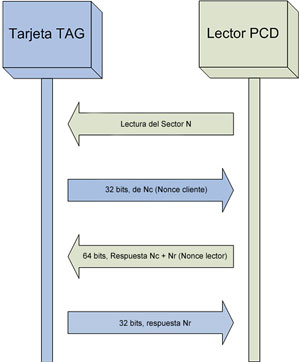
\includegraphics[width=0.6\textwidth]{figures/protocolo.jpg}
	\caption{Proceso de handshake de las tarjetas Mifare}
\end{figure}


Al comenzar lector le comunica a la tarjeta que quiere realizar una operación sobre un sector de datos determinado N. El tag o tarjeta en ese momento remite un número aleatorio Nc (Nonce del cliente) de 32 bits a modo de reto, para que sea cifrado con la clave privada compartida previamente. Como respuesta, el lector remite el reto cifrado y un número aleatorio Nr (Nonce del lector) para que el tag lo cifre con la clave privada, generando una trama de 64 bits. En última instancia la tarjeta le envía al lector su reto cifrado. En este momento ambos tienen la certeza de que los dispositivos son legítimos. Destacar que los dos últimos intercambios se realizan ya de forma cifrada, permaneciendo en claro tan solo el envío de la petición de lectura y Nc.\\

Posteriormente necesitaríamos una tarjeta Mifare y un lector NFC conectado a un ordenador con el que posteriormente podremos ver los tags de la tarjeta. Colocando el sniffer entre la tarjeta y el lector podríamos proceder a realizar una lectura del sector 4, obteniendo la siguiente traza de bytes.

\begin{figure}[!h]
	\centering
	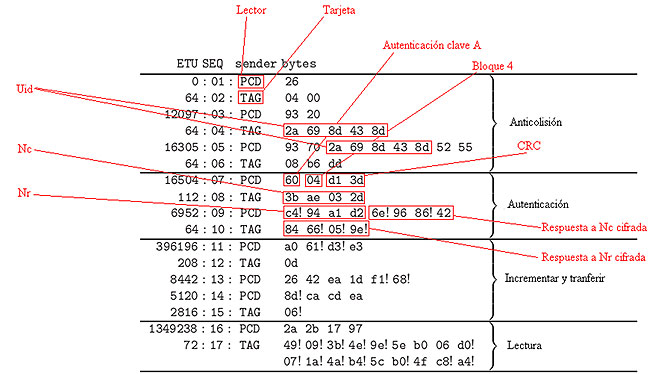
\includegraphics[width=0.8\textwidth]{figures/lectura.jpg}
	\caption{Lectura de la tarjeta Mifare}
\end{figure}

Con la información que hemos capturado podremos intervenir la clave privada del sector mediante una aplicacion llamada \textit{CRAPTO1}. \\

Con esta clave privada ya podremos leer/modificar el contenido de los bloques de datos que componen el sector 01. Podríamos por ejemplo incrementar el valor del monedero electrónico, si el valor reside dentro de la tarjeta. Lo mas habitual es encontrarse el reste de sectores protegidos con la misma pk, lo que habilitaría un clonado completo de la tarjeta.

\subsection{Conclusión}

Los microcontroladores son una solución mas viable que las aplicaciones que se puedan crear para Android ya que los microcontroladores se hacen expresamente para esto y en cambio en Android tienes que ceñirte a la API que este te ofrece. En cambio, los microcontroladores requieren conocimientos de electrónica avanzados a parte de saber como programarlos.



